\chapter{PROJECT MANAGEMENT PLAN}

%------------------------------------------------------------------
% Schedule — Gantt Chart
%------------------------------------------------------------------
\section{Schedule of the Project}

\begin{spacing}{1.5}
The project ran from January 2026 to June 2026 across ten two-week sprints. The timeline below reflects the actual sequence of work undertaken, from initial literature review through to final report submission.
\end{spacing}

\begin{figure}[H]
\centering
\resizebox{\textwidth}{!}{%
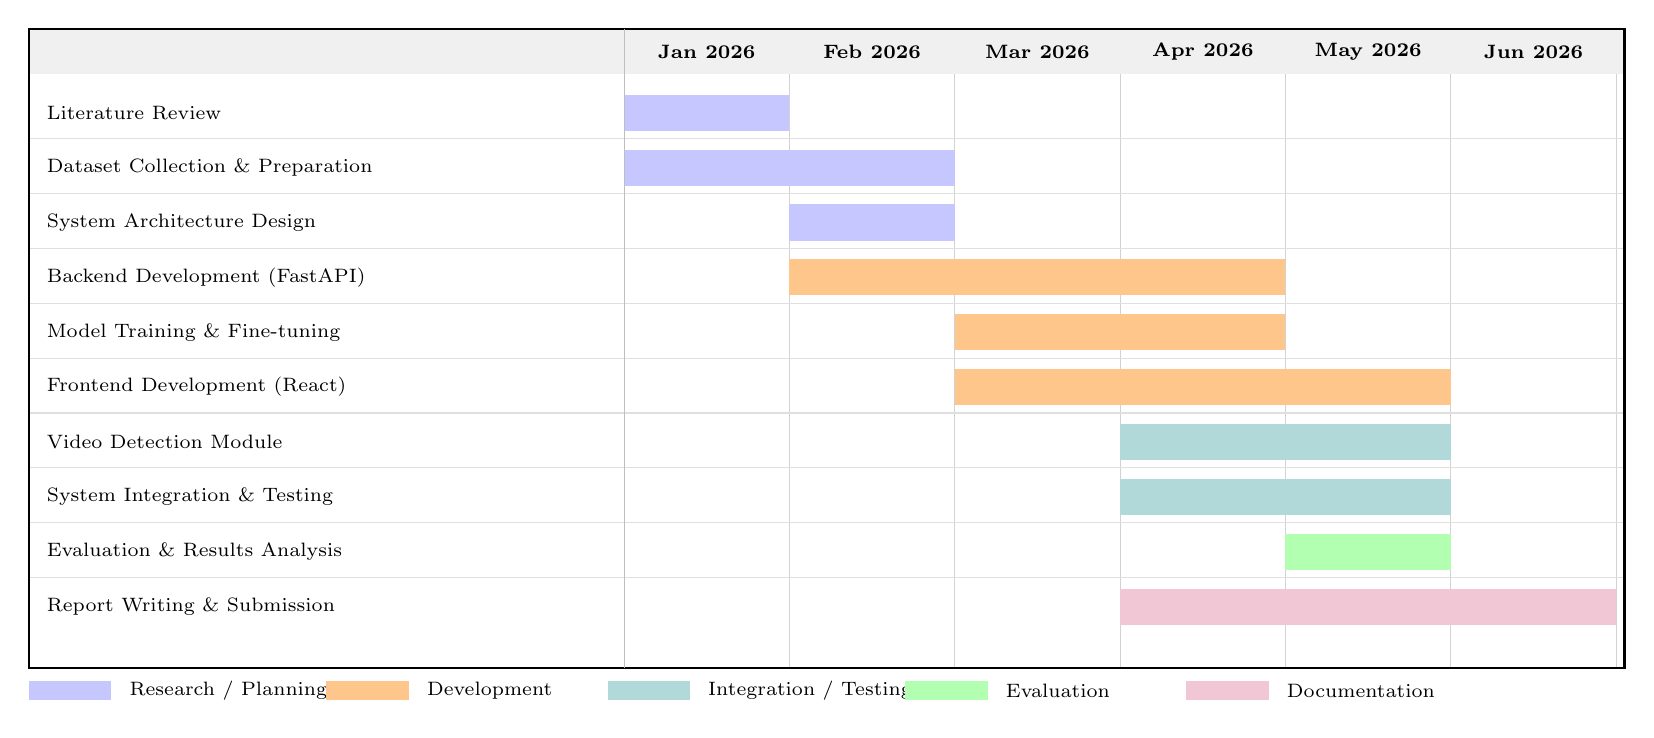
\begin{tikzpicture}[x=2.1cm, y=0.82cm, font=\small]

  % ── Month header background ──────────────────────────────────────
  \fill[gray!12] (-3.6, 0.15) rectangle (6.05, 0.85);

  % ── Month labels ─────────────────────────────────────────────────
  \foreach \x/\mo in {0/Jan,1/Feb,2/Mar,3/Apr,4/May,5/Jun}{
    \node[font=\scriptsize\bfseries] at (\x+0.5, 0.5) {\mo\ 2026};
  }

  % ── Vertical grid lines ───────────────────────────────────────────
  \foreach \x in {0,1,2,3,4,5,6}{
    \draw[gray!35, thin] (\x, 0.15) -- (\x, -9.05);
  }

  % ── Task rows  (label | bar-start | bar-end | fill) ───────────────
  % Row centres at y = -0.45, -1.30, -2.15, -3.00, -3.85, -4.70, -5.55, -6.40, -7.25, -8.10
  % Bar half-height = 0.28

  % 1. Literature Review  Jan
  \node[anchor=west, font=\scriptsize] at (-3.55,-0.45) {Literature Review};
  \fill[blue!22]   (0,-0.17) rectangle (1,-0.73);

  % 2. Dataset Collection  Jan – Feb
  \node[anchor=west, font=\scriptsize] at (-3.55,-1.30) {Dataset Collection \& Preparation};
  \fill[blue!22]   (0,-1.02) rectangle (2,-1.58);

  % 3. Architecture Design  Feb
  \node[anchor=west, font=\scriptsize] at (-3.55,-2.15) {System Architecture Design};
  \fill[blue!22]   (1,-1.87) rectangle (2,-2.43);

  % 4. Backend Development  Feb – Apr
  \node[anchor=west, font=\scriptsize] at (-3.55,-3.00) {Backend Development (FastAPI)};
  \fill[orange!45] (1,-2.72) rectangle (4,-3.28);

  % 5. Model Training  Mar – Apr
  \node[anchor=west, font=\scriptsize] at (-3.55,-3.85) {Model Training \& Fine-tuning};
  \fill[orange!45] (2,-3.57) rectangle (4,-4.13);

  % 6. Frontend Development  Mar – May
  \node[anchor=west, font=\scriptsize] at (-3.55,-4.70) {Frontend Development (React)};
  \fill[orange!45] (2,-4.42) rectangle (5,-4.98);

  % 7. Video Detection  Apr – May
  \node[anchor=west, font=\scriptsize] at (-3.55,-5.55) {Video Detection Module};
  \fill[teal!30]   (3,-5.27) rectangle (5,-5.83);

  % 8. Integration \& Testing  Apr – May
  \node[anchor=west, font=\scriptsize] at (-3.55,-6.40) {System Integration \& Testing};
  \fill[teal!30]   (3,-6.12) rectangle (5,-6.68);

  % 9. Evaluation \& Results  May
  \node[anchor=west, font=\scriptsize] at (-3.55,-7.25) {Evaluation \& Results Analysis};
  \fill[green!30]  (4,-6.97) rectangle (5,-7.53);

  % 10. Report Writing  Apr – Jun
  \node[anchor=west, font=\scriptsize] at (-3.55,-8.10) {Report Writing \& Submission};
  \fill[purple!22] (3,-7.82) rectangle (6,-8.38);

  % ── Horizontal dividers ───────────────────────────────────────────
  \foreach \y in {-0.85,-1.70,-2.55,-3.40,-4.25,-5.10,-5.95,-6.80,-7.65}{
    \draw[gray!25, thin] (-3.6,\y) -- (6.05,\y);
  }

  % ── Outer border ─────────────────────────────────────────────────
  \draw[thick] (-3.6, 0.85) rectangle (6.05, -9.05);
  \draw[gray!50] (0, 0.85) -- (0, -9.05);   % label / chart divider

  % ── Legend ───────────────────────────────────────────────────────
  \fill[blue!22]   (-3.6,-9.55) rectangle (-3.1,-9.25);
  \node[anchor=west,font=\scriptsize] at (-3.05,-9.40) {Research / Planning};
  \fill[orange!45] (-1.8,-9.55) rectangle (-1.3,-9.25);
  \node[anchor=west,font=\scriptsize] at (-1.25,-9.40) {Development};
  \fill[teal!30]   (-0.1,-9.55) rectangle (0.4,-9.25);
  \node[anchor=west,font=\scriptsize] at (0.45,-9.40) {Integration / Testing};
  \fill[green!30]  (1.7,-9.55) rectangle (2.2,-9.25);
  \node[anchor=west,font=\scriptsize] at (2.25,-9.40) {Evaluation};
  \fill[purple!22] (3.4,-9.55) rectangle (3.9,-9.25);
  \node[anchor=west,font=\scriptsize] at (3.95,-9.40) {Documentation};

\end{tikzpicture}
}
\caption{Project Gantt Chart --- January to June 2026}
\label{fig:gantt}
\end{figure}

%------------------------------------------------------------------
% Risk Identification
%------------------------------------------------------------------
\section{Risk Identification}

\begin{spacing}{1.5}
Table~\ref{tab:risks} lists the key risks identified at the start of the project, along with their likelihood, impact, and the mitigation strategy applied. Several of these risks materialised during development --- most notably the dataset access issue --- and the mitigations described reflect what was actually done rather than theoretical contingency plans.
\end{spacing}

\renewcommand{\arraystretch}{1.35}
\begin{table}[H]
\centering
\begin{tabular}{|p{3.4cm}|c|c|p{6.2cm}|}
\hline
\textbf{Risk} & \textbf{Likelihood} & \textbf{Impact} & \textbf{Mitigation} \\
\hline
Research datasets unavailable (CelebDF-v2, FaceForensics++) & High & High &
  Submitted formal access requests early; fell back to Kaggle and HuggingFace datasets when access was not granted before deadline \\
\hline
Model accuracy below acceptable threshold & Medium & High &
  Used a three-model ensemble so no single model failure is catastrophic; monitored AUC-ROC during training and used progressive unfreezing for F3Net \\
\hline
GPU compute constraints & Medium & Medium &
  Used Kaggle free-tier GPU (T4, 30 h/week); designed the pipeline to run on CPU by default so development was not blocked \\
\hline
Frontend--backend integration failures & Low & Medium &
  Agreed on API schema (request/response JSON) before writing either side; used Vite's built-in proxy to avoid CORS issues in development \\
\hline
Scope creep & Medium & Medium &
  Explicitly excluded reverse image search and real-time video streaming from scope at the start; tracked work in sprint tickets \\
\hline
Key dependency deprecation & Low & Low &
  Pinned library versions in \texttt{requirements.txt} and \texttt{package.json}; avoided unstable pre-release packages \\
\hline
\end{tabular}
\caption{Risk Identification and Mitigation}
\label{tab:risks}
\end{table}
